
\section{KIDs specific systematics and application to CMB polarization}

In view of future utilizations of KIDs in space mission it is necessary to demonstrate the capabilities and the suitability of KIDs arrays in a space like environment. In this section we will adress some of the systematics effects that need to be taken into account during the design of futur generation detector arrays for space applications, such as the KIDs non-linearity. Here we describe the simulation method used to study the KIDs non-linearity, then we will study the KIDs linearity for different sources... \\

\subsection{Simulations}
To adress the KIDs non-linearity, we do simulations of their response to an incoming source of radiation using \rf and \cf. In this section, we give an explanation of the used method and its results.

	\subsubsection{Method}
	
The simulation method consists in modelling the response of a KID to a scan of a bright source, then to reconstruct the signal with the two methods described in Sec.\ref{sec:signal}.

\begin{figure}[h]
\center
\includegraphics[scale=0.55]{Figures/planets.eps}
\caption{Comparison of the incoming flux (in black) with the signals reconstructed by using \rf (in blue) and \cf (in red). In the top pannel and bottom pannels, the incoming fluxes are respectively $10^{4}$ and $10^{5}$ Hz.}
\label{fig:planets}
\end{figure}

\begin{figure}[h]
\center
\includegraphics[scale=0.8]{Figures/resonance.eps}
\caption{Simulation of a resonance in the $I-Q$ plane, for incoming fluxes equal to $10^{4}$ (in red) and $10^{5}$ (in black) Hz.}
\label{fig:resonance}
\end{figure}

Fig.\ref{fig:planets} represents the reconstructed signal with different incoming flux. We observe that at a higher flux, the signal is less well reconstructed by \rf. Fig. \ref{fig:resonance} represents the corresponding sweep of $I-Q$ around the resonance.

In order to derive the KID non-linearity, we do a gaussian fit of the outcoming signal, to be able to plot the incoming flux as a function of the outcoming flux. This function is then fitted by a parabola :

\begin{equation}
\phi_{out} = \alpha \phi_{in} + \beta \phi_{in}^{2} ,
\label{eq:fit-nl-1}
\end{equation}

\begin{equation}
\phi_{out} = \alpha (\phi_{in} + \frac{\beta}{\alpha}  \phi_{in}^{2}).
\label{eq:fit-nl-2}
\end{equation}

The coefficient $\alpha$ is not fixed, but will be absorbed by the calibration. Eq \ref{eq:fit-nl-2} becomes :

\begin{equation}
\phi_{out} = \phi_{in} + \varepsilon \phi_{in}^{2},
\label{eq:fit-nl-3}
\end{equation}

with $\varepsilon = \frac{\beta}{\alpha}$ the non-linearity coefficient. \\
In the following paragraph, we will use the model described by Eq \ref{eq:fit-nl-3} to study the KID non-linearity when it is exposed to different sources such as : a planet, the CMB dipole, and a half wave plate (HWP).

\subsubsection{KIDs non-linearity}

The KIDs linearity has been demonstrated, over a large power range, in laboratory under realistic conditions as shown in Fig. \ref{KID-lin}. As we can see, at 300K the response of the KID is still under a linear regime.

\begin{figure}[h]
\center
	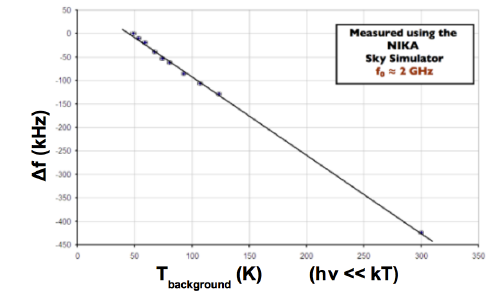
\includegraphics[scale=0.55]{Figures/KID-linearity-Monfardini2014.png}
	\caption{KID linarity demonstrated in laboratory under realistic conditions. Y-axis : frequency shift of the resonance (KID measured signal), X-axis : optical background temperature. The solid line represents the linear fit of the experimental points. Credits : \citet{2014JLTP..176..787M}.}
	\label{KID-lin}
\end{figure}

In the next paragraphs we do several simulations following the method described earlier. In these simulations we do a scanning strategy that ensures that the scanning speed is such that the number of points per beam is between 3 and 5 so that we respect Nyquist.

%\begin{figure}[h]
%\center
%	\includegraphics[scale=0.5]{Figures/nl_all.eps}
%	\caption{Output flux as a function of Input flux in Jy. The input signal corresponds to : a planet, planet and dipole, planet and HWP, planet, HWP and dipole, represented respectively by : cross, diamond, triangle, square. Blue :\rf reconstruction method, Red : \cf reconstruction method.}
%	\label{fig:nl-all}
%\end{figure}

\paragraph{Planet only \\}

Here we simulate the scan of a planet by a KID to see if the input signal is linearly reconstruted.

\begin{figure}[h]
\center
	\includegraphics[scale=0.5]{Figures/NL-planet.eps}
	\caption{Output flux as a function of Input flux in Jy. 
	The input signal corresponds to a planet. Cross and diamond represent the signal reconstructed respectively by \cf and \rf. Black : Output flux as a function of Input flux in Jy. Blue : Scan with 3 points per beam. Red : Scan with 5 points per beam.}
	\label{fig:nl-planet}
\end{figure}

Fig.\ref{fig:nl-planet} shows the output signal, reconstructed by \rf and \cf, as a function of the input signal at different fluxes. The signal is linearly reconstructed with \rf and \cf, but becomes non-linear at higher fluxes, especially for \rf.  \\

 \begin{table}[h!]
\center
	\begin{tabular}{|c|c|c|}
  	\hline
 	\backslashbox{$npts/fwhm$}{$\varepsilon$} & $	\varepsilon_{R_{f}}$ & $\varepsilon_{C_{f}} $ \\
	\hline
 	3  & - 8.05 x $10^{-5}$ & 3.78 x $10^{-7}$ \\
  	\hline
 	5 & 7.27 x $10^{-5}$ & 1,74 x $10^{-7}$ \\
  	\hline
	\end{tabular} 
\caption{Non-linearity coefficients \eps for \rf and \cf. The incoming flux corresponds to a planet (700 Jy).}
\label{tab:eps-planet}
\end{table} 

In the next parts we will see how this non-linearity progresses if we add other sources to the planet such as the CMB dipole and/or a HWP.

\paragraph{Planet and the CMB dipole \\}

The CMB dipole is a smooth gradient in the CMB temperature accross the sky. It is the result of the motion of the local group of galaxies with respect to the reference framed defined by the CMB. The CMB dipole amplitude is $\Delta T = 3.365 \pm 0.027$ mK and directed toward $(l,b) = (264.4 \degree \pm 0.3 \degree , 48.4 \degree \pm 0.5 \degree)$ in galactic coordinates \citep{2015IJMPD..2430004B}. Here we do a simulation with two incoming fluxes : a planet and the CMB dipole. 

\begin{figure}[h]
\center
	\includegraphics[scale=0.5]{Figures/NL-planet-dipole.eps}
	\caption{Output flux as a function of Input flux in Jy. 
	The input signal corresponds to a planet and the CMB dipole. Cross and diamond represent the signal reconstructed respectively by \cf and \rf. Blue : Scan with 3 points per beam. Black : Output flux as a function of Input flux in Jy. Red : Scan with 5 points per beam.}
	\label{fig:nl-planet-dipole}
\end{figure}

\begin{table}[h!]
\center
	\begin{tabular}{|c|c|c|}
  	\hline
 	\backslashbox{$npts/fwhm$}{$\varepsilon$} & $	\varepsilon_{R_{f}}$ & $\varepsilon_{C_{f}} $ \\
	\hline
 	3  & - 8.07 x $10^{-5}$ & 3.74 x $10^{-7}$ \\
  	\hline
 	5 & 7.29 x $10^{-5}$ & 1,73 x $10^{-7}$ \\
  	\hline
	\end{tabular} 
\caption{Non-linearity coefficients \eps for \rf and \cf. The incoming flux corresponds to a planet (700 Jy) and the CMB dipole.}
\label{tab:eps-planet-dipole}
\end{table}

Fig. \ref{fig:nl-planet-dipole} and Tab. \ref{tab:eps-planet-dipole} shows that like in the precedent simulation, the signal is well reconstructed at lower fluxes but becomes non-linear at higher fluxes notably with \rf. Plus, we can see that the more number of points per beam we have the smaller \eps becomes. 

%Fig \ref{fig:nl-planet-dipole} shows that the difference between the input signal and the output signal, and \eps, are of the same order as the ones in the simulation with only a planet, so adding the CMB dipole to the simulations does not bias the signal linearity. 

\paragraph{Planet, HWP and CMB dipole \\}

In this paragraph we do the same simulation but this time we add the signal of a HWP template to the incoming signals already consisting of a planet at 700 Jy and the CMB dipole.\\
Many experiments, such as MAXIPOL \citep{2007ApJ...665...42J}, EBEX \citep{2010SPIE.7741E..1CR}, POLARBEAR \citep{2017JCAP...05..008T}, \nika2 \citep{2017A&A...599A..34R}, use half-wave plates (HWPs) to improve the sensitivity in polarization measurements by reducing instrumental systematics errors and low-frequency noise. Plus, it allows independant measurements of the three Stokes parameters : I, Q, and U. However, by implementing a HWP, we need to address several issues such as intensity to polarisation leakage and additional parasitic signal peaked at harmonics of the HWP rotation frequency brought by imperfections of the HWP.

\begin{figure}[h]
\center
	\includegraphics[scale=0.5]{Figures/NL-planet-hwp-dipole.eps}
	\caption{Output flux as a function of Input flux in Jy. 
	The input signal corresponds to a planet, the CMB dipole and a HWP template. Cross and diamond represent the signal reconstructed respectively by \cf and \rf. Black : Output flux as a function of Input flux in Jy. Blue : Scan with 3 points per beam. Red : Scan with 5 points per beam.}
	\label{fig:nl-planet-hwp-dipole}
\end{figure}

\begin{table}[h!]
\center
	\begin{tabular}{|c|c|c|}
  	\hline
 	\backslashbox{$npts/fwhm$}{$\varepsilon$} & $	\varepsilon_{R_{f}}$ & $\varepsilon_{C_{f}} $ \\
	\hline
 	3  & - 8.99 x $10^{-5}$ & -2.58 x $10^{-7}$ \\
  	\hline
 	5 & 7.50 x $10^{-5}$ & 1,54 x $10^{-7}$ \\
  	\hline
	\end{tabular} 
\caption{Non-linearity coefficients \eps for \rf and \cf. The incoming flux corresponds to a planet (700 Jy), a HWP template and CMB dipole.}
\label{tab:eps-planet-hwp-dipole}
\end{table}

Like in the two precedent simulations we can see in Fig. \ref{fig:nl-planet-hwp-dipole} and Tab. \ref{tab:eps-planet-hwp-dipole} that the signal is well reconstructed but that non-linearities appear at higher fluxes. We note that, compared to the simulation with only the planet, the non-linearity brought by the HWP is negligeable.\\

\begin{figure}[h]
\center
	\includegraphics[scale=0.5]{Figures/diff-planet-hwp-dipole-rf.eps}
	\caption{Difference between the output and input signals as a function of the input signal (Jy). Signal were reconstructed with \rf. Diamond, triangle, square and cross correspond respectively to a planet, planet and dipole, planet and HWP template, planet and dipole and HWP template. Blue : Scan with 3 points per beam. Red : Scan with 5 points per beam.}
	\label{fig:diff-rf}
\end{figure}

\begin{figure}[h]
\center
	\includegraphics[scale=0.5]{Figures/diff-planet-hwp-dipole-cf.eps}
	\caption{Difference between the output and input signals as a function of the input signal (Jy). Signal were reconstructed with \cf. Diamond, triangle, square and cross correspond respectively to a planet, planet and dipole, planet and HWP template, planet and dipole and HWP template. Blue : Scan with 3 points per beam. Red : Scan with 5 points per beam.}
	\label{fig:diff-cf}
\end{figure}

Fig. \ref{fig:diff-rf} and Fig. \ref{fig:diff-cf} supports the fact that there are less non-linearities brought by the way that we reconstruct the signal when we do a scan over more points per beam... and that \cf is less limited at higher flux than \rf.\\ 

To conclude, we can say that both methods \rf and \cf linearly reconstruct the signal even if they become limited at higher flux. Still, the non-linearity coefficients derived by \cf ($\sim 10^{-7}$) are lower than those found with \rf ($\sim 10^{-5}$), meaning that \cf is better than \rf even if it already reconstructed the signal very well.
Plus, we saw that adding a HWP template to an incoming signal consisting of a planet and the CMB dipole only slightly adds non-linearity to the signal and so does not bias the linearity of the signal reconstruction. Moreover, to be able to reconstruct the signal well, we need to put constraints on the scanning speed and so the number of points per beam. In order to do that, the following paragraph,  we study realistic simulations by using a scanning strategy typical of a satellite to scan the Galaxy.


\subsubsection{Scanning strategy : Pol sat, PLANCK}
A key factor in the design of space experiments is the scanning strategy of the instrument, as it will play a role in the systematics effect that comes from the instrument. Here, we present different simulations of scanning strategies such as the ones used in EPIC \citep{2009arXiv0906.1188B}, and PLANCK \citep{2005A&A...430..363D}.

\paragraph{Pol sat \\}
For Pol sat's scanning strategy, the optical axis of the telescope is inclined by 55 $\degree$ with respect to the spin axis The spin axis is inclined by 45 $\degree$ from the precession axis and it precesses around the Sun-Earth axis every hour.

\paragraph{PLANCK \\}
PLANCK scans large circles on the sky with a 85 $\degree$ angle between the optical axis and the spin axis. The precession angle is 7 $\degree$.

\begin{figure}[h]
\center
	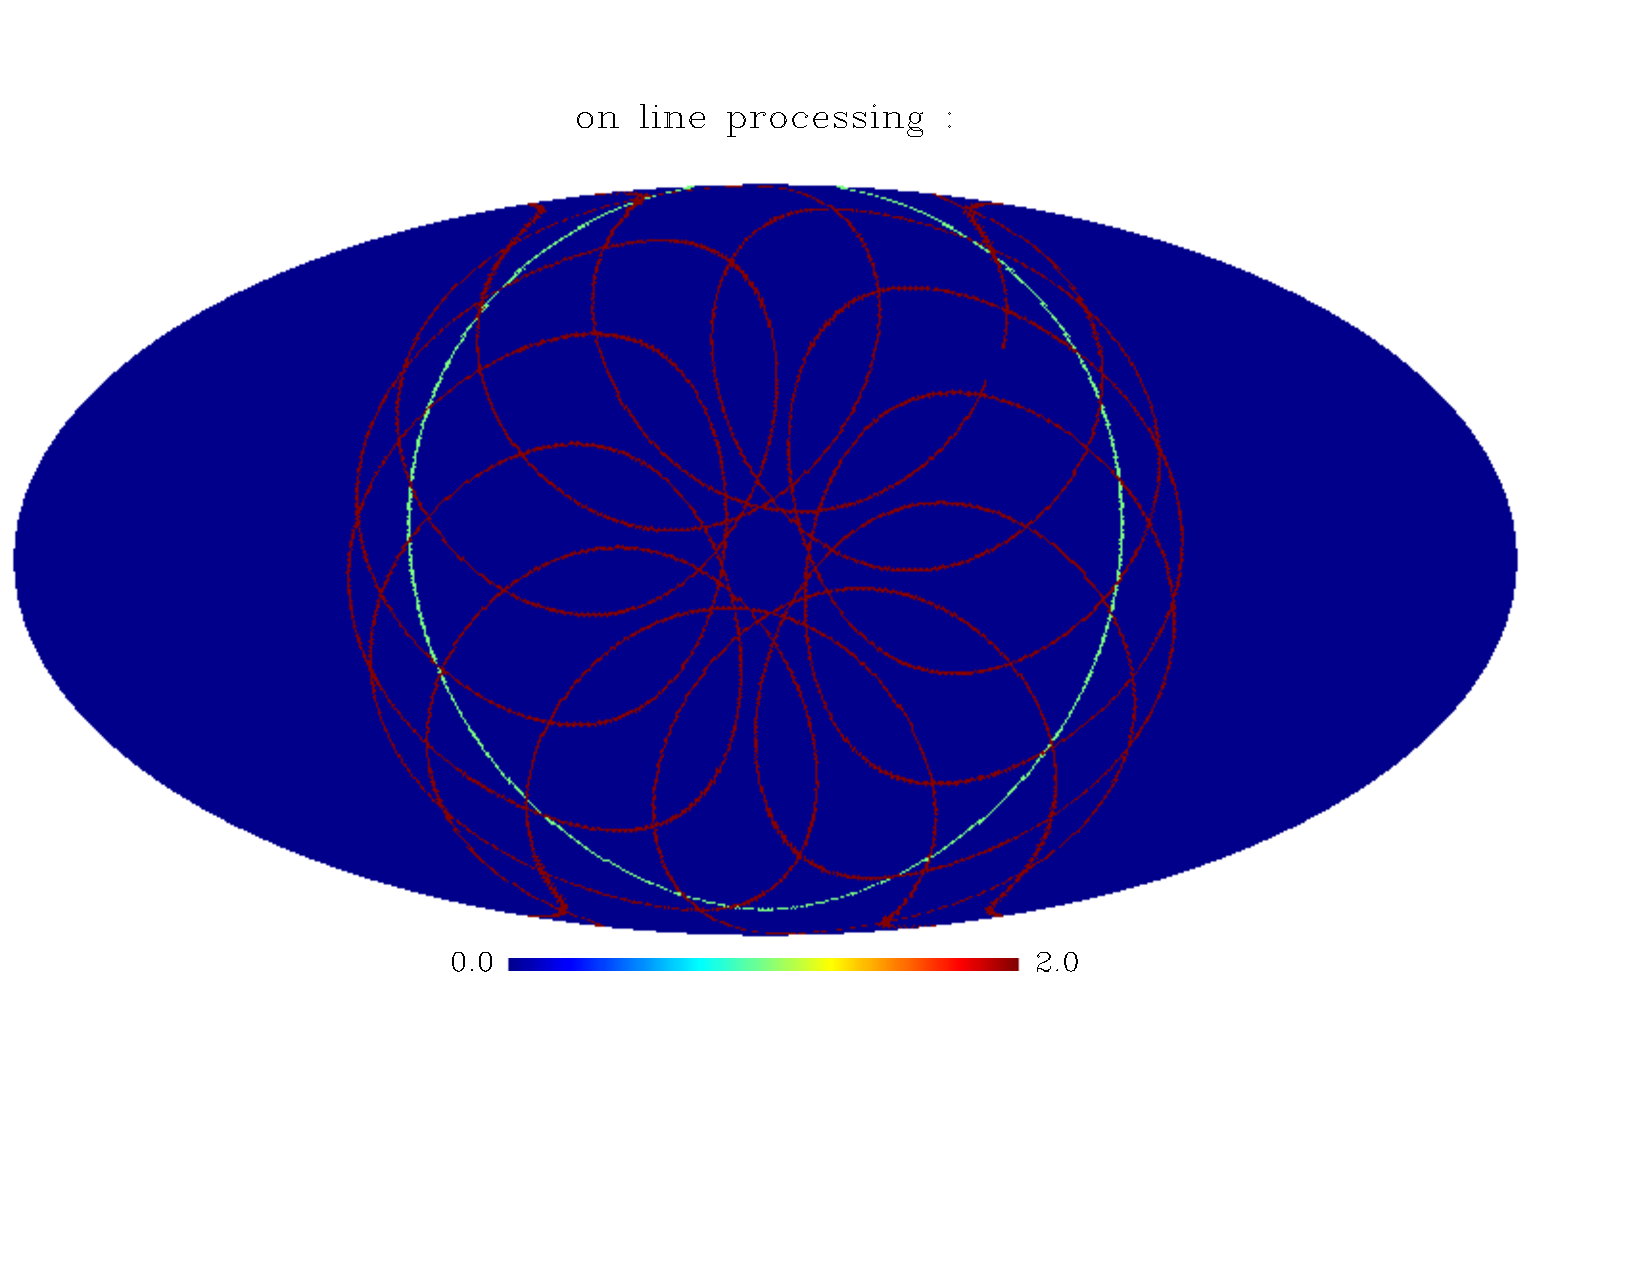
\includegraphics[scale=0.3]{Figures/scan_strat_planck_polsat.pdf}
	\caption{Red : representation of Pol sat's scanning strategy. Green : representation of PLANCK's scanning strategy }
	\label{fig:strat_polsat}
\end{figure}

In the next paragraph we will do a more realistic simulation by scanning a map of the Galaxy (REF) and the cosmological dipole with a HWP, and by using these pointing strategies. 

\subsubsection{Results}

In order to derive the non-linearity coefficient in more realistic simulations we scan a map of the Galaxy and the dipole with the two pointing strategies described earlier. Like in the precedent simulations we add the template of a HWP that we subtract after the signal goes through the KID model.

\paragraph{Pol sat \\}

\begin{figure}[h]
\center
	\includegraphics[scale=0.5]{Figures/toi-galaxy-dipole.eps}
	\caption{Representation of the incoming flux (Galaxy and Dipole in black), scanned by Pol sat, and its reconstruction. Red : Reconstruction of the incoming signal using \cf. Blue : Reconstruction of the incoming signal using \rf.
}
	\label{fig:toi-galaxy-dipole-pol}
\end{figure}

\begin{figure}[h]
\center
	\includegraphics[scale=0.5]{Figures/NL-galaxy-dipole.eps}
	\caption{Output flux as a function of Input flux (Galaxy and Dipole) in Jy. Red : The signal was reconstructed with \cf. Blue : The signal was reconstructed with \rf.}
	\label{fig:nl-galaxy-dipole-pol}
\end{figure}

Fig. \ref{fig:toi-galaxy-dipole} and  Fig. \ref{fig:nl-galaxy-dipole-pol} shows that the Galaxy and the dipole are well reconstructed by \rf and \cf. Plus, in Fig. \ref{toi-galaxy-hwp-dipole-pol} and Fig. \ref{fig:nl-galaxy-hwp-dipole-pol} we can see that the reconstructed signal is not strongly impacted by the HWP as the output signal is still very linear with the input signal.

\begin{figure}[h]
\center
	\includegraphics[scale=0.5]{Figures/toi-galaxy-hwp-dipole.eps}
	\caption{Representation of the incoming flux (Galaxy, Dipole and HWP in black), scanned by Pol sat, and its reconstruction. Red : Reconstruction of the incoming signal using \cf. Blue : Reconstruction of the incoming signal using \rf. }
	\label{fig:toi-galaxy-hwp-dipole-pol}
\end{figure}

\begin{figure}[h]
\center
	\includegraphics[scale=0.5]{Figures/NL-galaxy-hwp-dipole.eps}
	\caption{Output flux as a function of Input flux (Galaxy, Dipole and HWP) in Jy. Red : The signal was reconstructed with \cf. Blue : The signal was reconstructed with \rf.}
	\label{fig:nl-galaxy-hwp-dipole-pol}
\end{figure}

\begin{table}[h!]
\center
	\begin{tabular}{|c|c|c|}
  	\hline
 	\backslashbox{$Input signal$}{$\varepsilon$} & $	\varepsilon_{R_{f}}$ & $\varepsilon_{C_{f}} $ \\
	\hline
 	$G+D$  & -1.45 x $10^{-7}$ & -2.05 x $10^{-8}$ \\
  	\hline
 	$G+D+HWP$ & 3.54 x $10^{-4}$ & 3.06 x $10^{-7}$ \\
  	\hline
	\end{tabular} 
\caption{Non-linearity coefficients \eps for \rf and \cf. $G$, $D$ and $HWP$ respectively stands for Galaxy, Dipole and Half Wave Plate.}
\label{tab:eps-galaxy-hwp-dipole-pol}
\end{table}

\paragraph{Planck \\}

In this paragraph we do the same simulations but we use Planck's scanning strategy. 
Here again the input signals are linearly reconstructed by \rf and \cf without (cf Fig. \ref{fig:toi-galaxy-dipole-planck} and \ref{fig:nl-galaxy-dipole-planck}) or with (cf Fig. \ref{fig:toi-galaxy-hwp-dipole-planck} and \ref{fig:tnl-galaxy-hwp-dipole-planck}) the HWP.

\begin{figure}[h]
\center
	\includegraphics[scale=0.5]{Figures/toi-galaxy-dipole-planck.eps}
	\caption{Representation of the incoming flux (Galaxy and Dipole in black), scanned by PLANCK, and its reconstruction. Red : Reconstruction of the incoming signal using \cf. Blue : Reconstruction of the incoming signal using \rf.
}
	\label{fig:toi-galaxy-dipole-planck}
\end{figure}

\begin{figure}[h]
\center
	\includegraphics[scale=0.5]{Figures/NL-galaxy-dipole-planck.eps}
	\caption{Output flux as a function of Input flux (Galaxy, Dipole) in Jy. Red : The signal was reconstructed with \cf. Blue : The signal was reconstructed with \rf.}
	\label{fig:nl-galaxy-dipole-planck}
\end{figure}

\begin{figure}[h]
\center
	\includegraphics[scale=0.5]{Figures/toi-galaxy-hwp-dipole-planck.eps}
	\caption{Representation of the incoming flux (Galaxy, Dipole and HWP in black), scanned by PLANCK, and its reconstruction. Red : Reconstruction of the incoming signal using \cf. Blue : Reconstruction of the incoming signal using \rf. }
	\label{fig:toi-galaxy-hwp-dipole-planck}
\end{figure}

\begin{figure}[h]
\center
	\includegraphics[scale=0.5]{Figures/NL-galaxy-hwp-dipole-planck.eps}
	\caption{Output flux as a function of Input flux (Galaxy, Dipole and HWP) in Jy. Red : The signal was reconstructed with \cf. Blue : The signal was reconstructed with \rf.}
	\label{fig:nl-galaxy-hwp-dipole-planck}
\end{figure}

\begin{table}[h!]
\center
	\begin{tabular}{|c|c|c|}
  	\hline
 	\backslashbox{$Input signal$}{$\varepsilon$} & $	\varepsilon_{R_{f}}$ & $\varepsilon_{C_{f}} $ \\
	\hline
 	$G+D$  & 6.48 x $10^{-6}$ & -2.99 x $10^{-8}$ \\
  	\hline
 	$G+D+HWP$ & 6.55 x $10^{-6}$ & 2.73 x $10^{-7}$ \\
  	\hline
	\end{tabular} 
\caption{Non-linearity coefficients \eps for \rf and \cf derived by using Planck's scanning strategy. $G$, $D$ and $HWP$ respectively stands for Galaxy, Dipole and Half Wave Plate.}
\label{tab:eps-galaxy-hwp-dipole-planck}
\end{table}

In Tab. \ref{tab:eps-galaxy-hwp-dipole-pol} and Tab. \ref{tab:eps-galaxy-hwp-dipole-planck} we can see that as expected, for both pointing strategies the non-linearity coefficients are higher when we add the HWP to the input signal. In addition, they emphasize the fact that the \cf method of signal reconstruction is slightly better than \rf, which confirms what we saw with the planet simulation.\\

To conclude, we have seen that both signal reconstruction methods can reconstruct the signal very well at low fluxes but start to be limited at higher fluxes. The non-linearity coefficient that we derived from them are very low. In every simulations, adding a HWP template to the incoming signal can slighlty add some non-linearities but it doesn't biais the reconstructed signal.\\

In the next section we will see 

LIEN VERS LA PARTIE CL

\section{Application to CMB maps and power spectra estimations}
The measurement of CMB polarization, and especially the detection of B modes, is one of the major challenges in modern cosmology. In this paper, we show that the KIDs systematic effect such as the non-linearity does not affect them from detecting B modes.

In this section we look at the next order correction, meaning that we will focus on the non-linear term produced by the detector and the way that we reconstruct the signal. A measure done by the KID is defined by $m = T + P$, with $T$ and $P$ representing the temperature and polarization. The non-linearity is characterized  by the $\varepsilon$ coefficient in $ m = m_{1} + \varepsilon m_{1}^{2}$. We have : 

\begin{equation}
\begin{split}
m & = m_{1} +\varepsilon' (T+P)^{2} \\
 & = T + P + \varepsilon'(T^{2} + P^{2} + 2TP) 
\end{split}
\end{equation}

Therefore, knowing that $T=I$ and $P = Q\cos(2\alpha) + U \sin(2\alpha)$, the polarized equation with a non-linear term is given Eq. \ref{eq-NL}.

\begin{equation}
m  \simeq (I + \varepsilon' I^{2}) + (Q + 2\varepsilon' IQ) \cos(2\alpha) + (U + 2 \varepsilon' IU) \sin(2\alpha)
\label{eq-NL}
\end{equation}

The non-linear coefficient $\varepsilon'$ is induced by the detector and the method used to reconstruct the signal.

The non-linearity coefficient $\varepsilon'$ does not intervene in the pointing strategy, in fact it is a systematic effect of the instrument and as a consequence will always impact our measurments. \\
To take into account this effect we simulate CMB maps with a PLANCK pointing strategy (citer ref) which follows Eq. \ref{eq-NL}. We used the HEALPix package/Ring pixelization scg=heme of the sphere (REF) to create simulated maps and to estimate power spectra.

%For allmaps we use the HEALPix Ring pixelization scheme of the sphere (Gorski et al. 1999)
%The input CMB power spectra were created with CAMB (Lewis & Challinor 2011) and we used the HEALPix package (Gorski et al. 2005) to create simulated maps, and to estimate power spectra

Eq. \ref{eq-NL} is translated in the the power spectrum by Eq. \ref{eq-Cl}.

\begin{equation}
C_{l}^{s} \propto \varepsilon^{2} C_{l}^{TE},
\label{eq-Cl}
\end{equation}
Where $C_{l}^{s}$ is the systematic power spectra.\\

We generate I, Q, U maps from observed $C_{l}$ to which we apply the non-linear mapping described by Eq.\ref{eq-NL}. This will produce spurious polarization signals from which we can derive modified $C_{l}^{s}$ and $\varepsilon$ represented in Eq. \ref{eq-Cl}. We found :

\begin{equation}
\varepsilon^{2} \simeq 4.10^{-7}.
\label{epsilon}
\end{equation}

\begin{figure}[h]
\center
	\includegraphics[scale=0.55]{Figures/cl.eps}
	\caption{cl}
	\label{fig:cl}
\end{figure}

This non-linearity can lead to leakage of the CMB temperature signal into the polarization maps and consequently can induce spurious polarization signals which could prevent us from detecting B mode polarization. The leakage effect is represented by the coefficient $\varepsilon$ of Eq. \ref{eq-Cl}. As a result, to be able to detect B mode polarization, the non-linearity coefficient related to the signal reconstruction must be lower than $\varepsilon^{2} \simeq 4.10^{-7}$.

%To do so, we calculate the non-linearity coefficient $\varepsilon'$ given by Eq.\ref{eq-NL} with a tolerance on mode B contamination by generating I, Q, U maps from observed $C_{l}$. Then we apply the non linear mapping described by Eq.\ref{eq-NL}, this will generate spurious signal from which we derive modified $C_{l}$. 

\subsection{Cosmic rays impact on KIDs array}

One of the major problems for space based missions is the impact of an intense flux of high energy particles, referred to as Cosmic Rays (CR) on the detectors. Primary CR are produced by the Sun and by other galactic sources. They are mostly composed by protons (90\%), helium nuclei (9\%) and a few heavier nuclei and electrons (1\%). The CR spectrum is peaked aroud 200 MeV, thus the particles have sufficient energy to penetrate the detectors and give an unwanted signal. The Planck satellite \citep{2014A&A...571A..10P} has demonstrated that the impact of CR on the detectors are a key problem for space missions. Indeed, the glitches caused by CR can mask the real data and induce a loss of an important fraction of it.\\
Experiments have been done to construct a setup that allows to study the behavior of KIDs arrays under typical conditions of a space-borne observatory, and establish the compatibility of KIDs with a space environment \citep{2016A&A...592A..26C,2016SPIE.9914E..0NM}. When the detector is hit by a CR there is a lapse of time during which the sensor is 'blind' to the incoming scientific data. The length of this dead-time depends on the response time of the KID (time constant) which is determined by the quasi particle lifetime. \citet{2012ApPhL.100w2601M} have shown for KID, this time constant is equal to about tens of microseconds which is faster than bolometers (from 5-10 ms to 2s). This means that for the same CR hit, less data is lost when using KIDs arrays. Plus, the experiments have confirmed the fact that KID recover their initial state in less than 5 milliseconds. Finally, \citet{2016SPIE.9914E..0NM} concluded that the percent level of data loss per pixel by a KIDs array placed in a space environment is about 1 \% compared to 15 \% for Planck HFI bolometers.\\ The KID technology shows promising results for compatibility with a space-borne mission, as their extremely short glitch time constant permits to greatly reduce the data loss fraction due to CR impacts. 

